\documentclass[draft]{article}

\usepackage{graphicx}
\usepackage{hyperref} % this should always be the last package

\newcommand{\mytitle}{Multi-thread simulation of a large scale dynamical system}
\newtheorem{requirement}{Requirement}
\newcommand{\e}{\epsilon}
\newlength{\rulewidth}\setlength{\rulewidth}{0.4pt}
\newcommand{\myrule}{\noindent\rule{\textwidth}{\rulewidth}}

\title{\mytitle}
\date{2021}
\author{Diego Bellani\thanks{Student}\and Enrico Tronci\thanks{Supervisor}}

\hypersetup{
	pdfauthor={Diego Bellani},
	pdftitle={\mytitle},
	pdfsubject={Bachelor thesis},
	pdfkeywords={bachelor,thesis,programming},
	pdfproducer={LaTeX},
	pdfcreator={pdfLaTeX},
	pdfborder={0 0 0},
	pageanchor=false
}

% TODO:
% * devo citare il più possibile e fare ricerca sulle varie cose citate
% * devo integrare il vecchio documento in the "Methods" section, mentre lo
%   spiego posso parlare dell'approccio preso per passare da un insieme di
%   equazioni ad un programma funzionante, anche perché è dove la maggior parte
%   del lavoro è andato. Tutte le varie \section possono essere trasformate in
%   \subsection.
% * devo parlare del processo di ottimizzazione, come sono partito da
%   un'implemetazione banale e sono arrivato a quella corrente, passando per lo
%   skip delle celle, per la trasformazione del sin + cos e in fine per
%   l'introduzione  di OpenMP
% * devo parlare dello schema, fare il diagramma ER, e parlare della sbrodolata
%   di vincoli in FOL
% * devo dire che un possibile miglioramento del mio codice potrebbe essere
%   quello di mettere N e B in due array separati per velocizzare il look up di
%   N ma nessun miglioramento è stato misurato, quindi neanche la versione bit
%   array è stata provata
% * devo inserire la foto di un tipico incendio per poter introdurre
%   l'assunzione principale, ovvero che le celle in fiamme sono poche
% * devo includere delle metriche sul codice e.g. il numero di linee di codice
% * magari posso mettere il link alla repository su github.com
% * forse doveri parlare di cos'è POSIX

% ERRORI TROVATI:
% * la probabilità deterministica (si erano scordati di dirci quali termini
%   perturbare)
% * divisioni per zero
% * mancanza di unità di misura
% * funzioni senza definizioni e mal poste (gamma può dare al più tre output per
%   amor del vero)
% * non è stato specificato cosa fare sulle condizioni del bordo
% * la halting condition è stata detta solo alla fine, all'inizio non ce n'era
%   nessuna

\begin{document}

\begin{titlepage}
\pagenumbering{roman}
\maketitle

\begin{abstract}
In this intership report I describe how a software for large scale, high
performance, forest fire simulation was developed, starting from a model given
by a third party and ending in a functioning implementation. The tecnology used
are described toghether with the various problems faced during the development
process. Finally some possible improvements and future developments are
described at the end.
\end{abstract}

\tableofcontents
\listoffigures
\listoftables
\end{titlepage}

\pagenumbering{arabic}

\section{Introduction}%%%%%%%%%%%%%%%%%%%%%%%%%%%%%%%%%%%%%%%%%%%%%%%%%%%%%%%%%%

Firefighting in forests is a complex activity due to the limited availability of
means and resources. Therefore the intervention strategy have to consider the
possible evolution of the fire to make the best use of what is available.

The possible evolution of a fire can be charaterized with a mathematical model
and predictred with a faster-then-real-time simulation of said model. Given
this, actions can be taken ahead of time to minimize the damage caused by the
fire and maximize the fire extinction speed.

\subsection{Context}

This intership is part of a project called ``Satellite Driven Fire Simulator'',
financed by the region of Lazio, to aid firefighters fight put out forest fires.

This project is divided in four parts:

\begin{enumerate}
\item development of a mathematical model (done by Paola Russo of the Tor
Vergata university \cite{mod});
\item \label{enum:my_work} development of a software to run the mathematcal
model (done by me);
\item \label{enum:interaction} development of a user interface for inputung data
to the simulator and showing the results in a human readable fashion;
\item \label{enum:data} gathering the data from the field, this includes
geographic data from satellites \cite{cop} and meteorologic data from on field
sensors.
\end{enumerate}

\subsection{Motivations}

To make predictions possible a software has to be developed that can show the
evolution of forest fires ahead of time.

The original implementation was made in Microsoft
Excel\textsuperscript{\textregistered}, which is fine for prototyping but not
suitable for fast large scale simulations. Therefore a better implementation was
needed both for speed and user friendlyness.

For this purpose an Intel server running a Linux based operating system was
provided.

The usual tool we used for implementation of mathematical models, Modelica, did
not made the cut beacuse of its limitation regarding dinamically sized arrays
and the exponential (\textbf{I'm not shure I can say that it is exponential})
time taken by the optimization algorithm at the increasing of the size of the
simulation grid.

Libraries exists to develop cellular automata models \cite{calib2}, but with
generality comes a lost in performance.

This said Modelica was still a valuable tool for prototyping a small version of
the model before its real implementation.

\subsection{Contributions}

I have implemented from scratch the simulator dividing it in two parts a data
integration one and a model execution one. Given that other parts of the project
have still to be implemented the data integration part of my software can be
used to make this other parts comunicate between each other.

Regarding the model that was used to implement the software, some corrections
have been done to it, by me and my advisor (i.e. I have noticed the problems and
my advisor promptly reported them or cerrected them on his own).

\subsection{Related Work}

Given that the model was provided to my by an external source, and therefore not
developed by me, I am not in the position to cite work related to that.

On the implementation side of things no inspiration was taken by other
implementations of fire simulator, so the same thing as before applies

\subsection{Outline}

This report is divided in 5 main sections. The first reviews the necessary
background information necessary to understand the work done. The second one
talks about the mathematical model and than the methods used to implement it, in
a mostly theoretical/high level way. The third talks about the actual
implementation of the software. The fourth talks about the experimental activity
done with the working program and the fifth and final section talks about what
could be done better in the current implementation and in eventual future works.

\section{Background}%%%%%%%%%%%%%%%%%%%%%%%%%%%%%%%%%%%%%%%%%%%%%%%%%%%%%%%%%%%%

The work done in this internship revolves arround three topics in particular:
cellular automata, the relational data model \cite{codd} and multithreaded
programming.

For the implementation side 4 main technologies have been used: the C
programming language for the implementation of the model, the SQL language for
interfacing with the database, the POSIX shell to integrate the database with
the implementation of the model and the OpenMP compiler extensions for the
parallelization of the algorithm.

The next sub-sections are dedicated to introducing all those previously cited
topics and technologies.

\subsection{Cellular Automata}

A cellular automata is a discrete model of computation based on a grid of cells
each with a finite number of states. Each cell has a neighborhood associated
with it, and it it used together with some rules to calculate the next
generation.

A particularly famous cellular automata configuration is the one created by
John~H.~Conway called ``Game of Life'' \cite{gol} it is played on a rectangular
grid (or a thorus), the neighborhood of each cell are the 8 arround it (also
known as the Moore neighborhood) and each cell has two state alive or dead.
There are three rules, one that determines the survival of a cell, on the death
and one the birth.

Even such a simple celluar automata has many intresting features, one of which
is beeing Turing complete \cite{win}.

Cellular automata have found applications in various scientific fields
\cite{cellularbio}. Even in the modelling of fire evolutiona as this project
shows.

\subsection{Relational Data Model}

The relational data model is a data model proposed by Edgar~F.~Codd for database
management systems. As the name implies it is based on mathematical relations. A
database is a collection of relation of tuples each of wich is made of atomical
values, this can be viewed as a set of tables. In the years what `atomical'
values are is changed \cite{ordb}. In the modern days an atomical value can be
an array, a tree structure or ever a tuple (record or struct) itself. This while
beeing counter intuitive is done for performance and expressiveness reasons.

In the schema made for this project array ad tuples where used as atomic values
in fact.

\subsection{Multithreading}

Multithreading is a computer architecture term that indicates that a single CPU
has multiples `cores' on it, each one with its own computational capability.
This can be taken advantage by programs, because the work can be divided across
the cores and executed in parallel. This can lead to speed ups in the execution
time linear to the amout of cores on the CPU, but often is not that easy to
archive this improvements due to syncronization problems.

\subsection{C}

C is a system programming language developed as a successor to the B programming
language at Bell Labs by Dennis~M.~Ritchie that has become the primary
implementation language for UNIX-like operating systems kernels and utilities.

The language is standardized by ISO and the version used in this project is
called C11, except for the standard library and the POSIX system interfaces no
other libraries were used.

\subsubsection{OpenMP}

OpenMP stands for Open Multi-Processing, it comprises a series of compiler
extensions, environment variables and library functions, for the C, C++ and
Fortran programming languages, that enables multithreaded programming with
minimal source code modification.

\subsection{SQL}

SQL stands for Structured Query Language, and it is a domani specific language,
for quering, manipulating and defining relational data. It is the de fato
standard language used for interfacing with databases based on the relational
data model.

The version used in this project is called SQL\raisebox{0.04cm}{:}98.

\subsection{Shell}

The Bourne Shell \texttt{sh(1)} is a programming language used for interfacing
with UNIX-like operating system, first developed by Stephen~Bourne at Bell Labs
and then standardized by POSIX.

Other shells exists but this is the only standardized one and many of the other
ones have this as a subset, so it is easy to found in a system.

\section{Methods}%%%%%%%%%%%%%%%%%%%%%%%%%%%%%%%%%%%%%%%%%%%%%%%%%%%%%%%%%%%%%%%

The majority of time in this project was spent on refining the mathematical
model given to us. Not only by stating it in a precise way the math in the model
but also in deriving from it a set of implementable requirements, that were not
very clear in the beginnning, even though in retrospect seems obvious.

After this activity was terminated the creation of the database schema and the
implementation of the model was relatively straight foreward.

\subsection{Model \& Data}

I have divided the model discussion in two parts a short introduction to the
data used, and than a longer discussion abouth the math used where the data
used, introduced in precendence, is refined.

\subsubsection{Data}\label{sec:data}

Now let's briefly talk about the data that the simulation will have at its
disposal, succesivelly they will be described in a more precise way. The
simulation has two kinds of data at his disposal geographical, from satellite
\cite{cop}, and meteorological from meteo station in place. The zone is divided
in squares and each square has uniform data.

The geographical datas are: altimetry, forest kind, urbanization level, eventual
water presence and the ``carta natura'', the last one is currently unused.

The meteorological data are just wind speed and direction.

\subsubsection{Model}

To describe the evolution of forest fire the model is based on three simple
observations

\begin{enumerate}
\item a fire burns until there is fuel,
\item a fire consume fuel,
\item a fire can move to a neighboring area.
\end{enumerate}

After having divided a rectangular area in $L^* \times W^*$ squared cells, we
understand that of each cell, in row $i$ and column $j$, of the forest we care
about just two charateristics: the fuel quantity it it at a certain point in
time $B_{ij}(t)$ and the presence or not of a fire in said cell at a certain
point in time $N_{ij}(t)$, $N$ can assume only two values 0 for no fire and 1
for fire, we will call finction like this \emph{fire indicator functions}. Those
two functions will represent the \emph{state} of the cell at any point in time.

Next to describe the concept of movement of the fire to neighboring cells a
cellular automata aproach was used.

But first we have to consider that a fire coud have multiple triggering points
across time, for example when we consider arson, for this cases a simple notion
of initial state is not sufficient, we need a way to talk about the exogenus
input of the system, let's call it $u_{ij}(t)$, and it is a fire indicator
function.

We can formalize everything that we have said until now with those equations

\begin{eqnarray}
N_{ij}(0) &=& u_{ij}(0)\textrm{,}\\
B_{ij}(0) &=& \gamma_{ij}\textrm{,}\\
N_{ij}(t+1) &=& \cases{\max(V_{ij}(t), u_{ij}(t)), &if $\underbrace{B_{ij}(t)}_\textrm{fuel} > 0$;\cr
                       0, &else.}\\
B_{ij}(t+1) &=& \cases{\max(0, B_{ij}(t)-\beta_{ij}\tau), &if $\underbrace{N_{ij}(t)}_\textrm{fire} > 0$;\cr
                       B_{ij}(t), &else.}
\end{eqnarray}

Where $\gamma_{ij}$is the initial fuel quantity in a cell, $V_{ij}(t)$ is the
possibility that the fire moves in the current cell from a neighboring one
(figure \ref{fig:automata}), $\beta_{ij}$ is the fuel consumption speed in a
particular cell and $\tau$ is the time step.

\begin{figure}
\centering
\setlength{\unitlength}{0.7cm}
\begin{picture}(6,6)
	\newlength{\piccenter}
	\setlength{\piccenter}{3\unitlength}
	% Grid
	\thicklines
	\multiput(0,0)(2,0){4}{\line(0,1){6}} % columns
	\multiput(0,0)(0,2){4}{\line(1,0){6}} % rows

	% Arrays
	\thinlines
	\put(\piccenter,\piccenter){\vector(1,0){2}}
	\put(\piccenter,\piccenter){\vector(0,1){2}}
	\put(\piccenter,\piccenter){\vector(-1,0){2}}
	\put(\piccenter,\piccenter){\vector(0,-1){2}}
	\put(\piccenter,\piccenter){\vector(1,1){2}}
	\put(\piccenter,\piccenter){\vector(-1,1){2}}
	\put(\piccenter,\piccenter){\vector(1,-1){2}}
	\put(\piccenter,\piccenter){\vector(-1,-1){2}}

	% Black square
	\newlength{\side}
	\setlength{\side}{0.8\unitlength}
	\linethickness{\side}
	\newlength{\ypos}
	\setlength{\ypos}{\piccenter}
	\addtolength{\ypos}{-0.5\side}
	\put(\piccenter,\ypos){\line(0,0){\side}}
\end{picture}
\caption{Neighborhood of a cell.}
\label{fig:automata}
\end{figure}

Obviously the heart of this model is the function $V_{ij}(t)$, another fire
indicator functions that it is defined in the following way

\begin{eqnarray}
            V_{ij}(t) &=& \max\{\,Q_{ij}(\e_1, \e_2, t) \mid (\e_1, \e_2) \in \Gamma\,\}\textrm{,}\\
               \Gamma &=& \{\,(x, y) \mid x, y \in \{-1, 0, 1\}\,\}\textrm{,}\\
Q_{ij}(\e_1, \e_2, t) &=& \cases{1, &if $p_{ij}(\e_1, \e_2, t) N_{i+\e_1j+\e_2}(t) > \theta$;\cr
                                 0, &else.}\label{eq:probtest}
\end{eqnarray}

Where $p_{ij}(\e_1, \e_2, t)$ is the probability that the fire moves from the
neighbor cell $(i+\e_1, j+\e_2)$ to the current cell $(i,j)$, $\theta$ is the
fire propagation threshold.

\myrule

Let's suspend, for now, our discussion about the model to better describe the
data at our disposal, introdiced in section \ref{sec:data}.

The satellite puts at our disposal a series of data, described in the table
\ref{tab:geo}, the meaning of the values is described in the appendix
\ref{sec:desc}. However those data cannot be used as is in the model but have to
be ``refined'' with the following mathematical corrispondences.

\begin{table}
\centering
\begin{tabular}{|c|l|c|}
	\hline
	\textbf{Symbol} & \textbf{Name} & \textbf{Interval}\\
	\hline
	$G$ & Foreste & 0,1,2,255\\
	$U$ & Urbanizzazione & 0,\ldots,100,255\\
	$W1$ & Water1 & 0,\ldots,4,253,255\\
	$W2$ & \underline{Water2} & 0,1\\
	$P$ & Altimetria & 0,\ldots,4380\\
	\hline
\end{tabular}
\caption{Geographical data for the single cell.}
\label{tab:geo}
\end{table}

\begin{equation}\label{eq:height}
H_{ij} = \cases{1 + G_{ij}, &if $0 \leq G_{ij} \leq 2$;\cr
                  0, &if $G_{ij} = 255$.}
\end{equation}

is the medium height  of the vegetation in a cell,

\begin{equation}\label{eq:inhabitants}
A_{ij} = \cases{U_{ij}/100, &if $0 \leq U_{ij} \leq 100$;\cr
                0, &if $U_{ij} = 255$.}
\end{equation}

is the percentage of the cell that is inhabited,

\begin{equation}\label{eq:water}
W_{ij} = \cases{0, &se $W1_{ij} = 0$;\cr
                1, &se $W1_{ij} = 1$;\cr
                0.75, &se $W1_{ij} = 2$;\cr
                0.75, &se $W1_{ij} = 3$;\cr
                0.5, &se $W1_{ij} = 4$;\cr
                1, &se $W1_{ij} = 253$;\cr
                1, &se $W1_{ij} = 255$.}
\end{equation}

is the percentage of water present. Those last three values are needed to
calculate due valori

\begin{equation}
S_{ij} = H_{ij} \cdot (1-A_{ij}) \cdot (1-W_{ij})\textrm{,}\\
\end{equation}

that is the level of inflammability of the cell, notice that $A_{ij}$ decreases
it because inhabited zones are usually cementified, and

\begin{equation} % NOTE: 4000 is the average wood density
\gamma_{ij} = 4000(H_{ij}-A_{ij})\textrm{.}
\end{equation}

The average height of a cell $P_{ij}$, is the only value left unchanged.

Now that we have finished to talk about the data used from the satellite, we can
talk about how the meteorological data is used in the simulation i.e. the speed
and direction of the wind

\begin{eqnarray}
\mathcal{F}_{ij} &=& F_{ij} + F_{ij}0.2r_1\\
\mathcal{D}_{ij} &=& D_{ij} + D_{ij}0.2r_2
\end{eqnarray}

Where $r_1$ and $r_2$ are two random numbers drawn from a normal distribution
centered in 0 between 1 and -1.

Finally we can caluculate

\begin{equation}
\beta_{ij} = 60(1+\mathcal{F}_{ij}/10)\textrm{,}
\end{equation}

Of the values not mentioned in precendence in the model just $S_{ij}$, $P_{ij}$,
$\mathcal{F}_{ij}$ and $\mathcal{D}_{ij}$ will be used.

\myrule

Now that we know which data we have at our disposal, we ca finally define
$p_{ij}(\e_1, \e_2, t)$ from function \ref{eq:probtest}.

\begin{equation}\label{eq:prob}
p_{ij}(\e_1, \e_2, t+1) = k_0 S_{ij} C_{i+\e_1j+\e_2}(t) d(\e_1, \e_2) f_w f_P\textrm{,}
\end{equation}

where $k_0$ is an optimization parameter and

\begin{equation}\label{eq:combust}
C_{i+\e_1j+\e_2}(t+1) = \exp\left(-\frac{B_{i+\e_1j+\e_2}(t) - \gamma_{i+\e_1j+\e_2}^2/4}{\Delta}\right)\textrm{,}
\end{equation}

is the combustion state of the cell. The  value that $C$ can assume has the form
of a gaussian curve so that the maximum value is reached when half of the fuel
is burned.

\begin{equation}\label{eq:disom}
d(\e_1, \e_2) = \left(1-\frac{1}{2}|\e_1\e_2|\right)\textrm{,}
\end{equation}

is the disomogeneity factor at the border of cells. It can assume only two
values 1 and $1/2$, the first is asumed when the considered cell is above,
below, to the left or to the right of the current cell the second one, instead,
when the considered cell is on a diagonal. This is done to take into account the
fact that the fire transmits less to digonal neighbor, as shown in figure
\ref{fig:disom}.

\begin{figure} % TODO: fix nummber positioning
\centering
\setlength{\unitlength}{0.7cm}
\begin{picture}(6,6)
	\setlength{\piccenter}{3\unitlength}
	% Grid
	\thicklines
	\multiput(0,0)(2,0){4}{\line(0,1){6}} % columns
	\multiput(0,0)(0,2){4}{\line(1,0){6}} % rows

	\put(1,5){1/2}
	\put(3,5){1}
	\put(5,5){1/2}
	\put(1,3){1}
	\put(5,3){1}
	\put(1,1){1/2}
	\put(3,1){1}
	\put(5,1){1/2}

	% Black square
	\setlength{\side}{0.8\unitlength}
	\linethickness{\side}
	\setlength{\ypos}{\piccenter}
	\addtolength{\ypos}{-0.5\side}
	\put(\piccenter,\ypos){\line(0,0){\side}}
\end{picture}
\caption{Disomogeneity at the border of the cell.}
\label{fig:disom}
\end{figure}

\begin{equation}\label{eq:wind}
f_w = \exp\left(k_1 \mathcal{F}_{i+\e_1j+\e_2}\frac{\begin{array}{c}\e_1\cos(\mathcal{D}_{i+\e_1j+\e_2})\\
      +\\\e_2\sin(\mathcal{D}_{i+\e_1j+\e_2})\end{array}}{\sqrt{\e_1^2 + \e_2^2}}\right)
\end{equation}

is the wind contribution, where $k_1$ is its optimization parameter, at last

\begin{equation}\label{eq:slope}
f_P = \exp\left(k_2\arctan\left(\frac{P_{ij}-P_{i+\e_1j+\e_2}}{L}\right)\right)
\end{equation}

is the contribution given from the slope between two cells and $k_2$ is its
optimization parameter.

To conclude the description of the model we state the alting condition: the
simulation halts iff no fire has been transmitter to a neighboring cell in an
entire simulation step.

All global parameters of the model and the ones of the single cells have been
grouped in tables \ref{tab:globals} and \ref{tab:params}.

\begin{table}
\centering
\begin{tabular}{|c|l|c|}
	\hline
	\textbf{Symbol} & \textbf{Name} & \textbf{Unit of measure}\\
	\hline
	$\tau$ & time step & seconds\\
	$L$ & side length of a cell & meters\\
	$L^*$ & length of the simulated area & meters\textsuperscript{2}\\
	$W^*$ & width of the simulated area & meters\textsuperscript{2}\\
	$\Delta$ & height of the normal distribution & adimensional\\
	$\theta$ & propagation probability & adimensional\\
	$k_0$ & threshold optimization & adimensional\\
	$k_1$ & wind optimization & adimensional\\
	$k_2$ & slope optimization & adimensional\\
	\hline
\end{tabular}
\caption{Parameters valid for each cell.}
\label{tab:globals}
\end{table}

\begin{table}
\centering
\begin{tabular}{|c|l|c|}
	\hline
	\textbf{Symbol} & \textbf{Name} & \textbf{Unit of measure}\\
	\hline
	$H$ & medium height of the vegetation & meters\\
	$A$ & urbanization percentage & adimensional\\
	$W$ & percentage of water presence & adimensional\\
	$\beta$ & combustion speed & kilograms/second\\
	$\gamma$ & fuel quantity & kilograms\\
	$S$ & inflammability percentage & adimensional\\
	$P$ & medium height & meters\\
	$\mathcal{D}$ & wind direction & radiants\\
	$\mathcal{F}$ & wind speed & meters/second\\
	\hline
\end{tabular}
\caption{Parameters for single cells.}
\label{tab:params}
\end{table}

\subsection{Database Schema}\label{sec:schema}

The ER diagram for the database schema is shown in figure \ref{fig:er}. It is a
simple diagram where attributes have been omitted but are reported here.

\begin{figure} % TODO: to finish
\centering
\setlength{\unitlength}{1cm}
\begin{picture}(6,6)
\setlength{\fboxsep}{8pt}
\put(0,0){\fbox{Map}}
\put(1,1){\fbox{Simulation}}
\put(2,2){\fbox{Result}}
\put(3,3){Work in progress\dots}
\end{picture}
\caption{ER diagram}
\label{fig:er}
\end{figure}

\begin{itemize}
\item Map(\underline{id}, name, unit, rect, data)
\item Simulation(\underline{id}, name, rect, map, horizon, ``snapshot freq'',
seed, Delta, tau, theta, k0, k1, k2, L, started)
\item Result(\underline{sim}, \underline{seq}, data)
\end{itemize}

The `data' attribute in Map is an array of tuples containing all the data,
meteorological and geographical, of the single cells discussed before, the
`data' attibute in Result is an array tuples containing the state of the cell
i.e. the presence of fire and the amount of fuel in it. `rect' in both Map and
Simulation is a pair of points that in the first one indicates where on the
globe, in the LAEA\footnote{Proiezione Lambert azimuthal Equal-Area} Europe
\cite{laeae} coordinate system with referiment system ETRS89\footnote{European
Terrestrial Reference System} \cite{etrs89}, the map is situated. The second one
indicates which subset of the map the simulation has been run on.

The use of the `unit' attribute in the Map entity indicates which multiple of
meters the points in `rect' are, this ensures that every possible coordinate is
in the correct multiple of digit, because the points in `rect' are stored as
integers.

Obviously the various arrays and rectangles have to be kept in check to avoid
incosistend database state, using the ER semantic of Toni Mancini \cite{bd2}
let's express the non-trivial contrains on the data first in natural language
and then in fist order logic.

\begin{enumerate}
\item In Simulation the area of rect must be the same as the length of data,
\item the area of data in Result must be the same of the rect of its Simulation,
\item the rect of Map must contain the on of each Simulation on it
\item the seq attribute of Result must be a sequence of increasing numbers
starting from zero
\end{enumerate}

\begin{enumerate}
\item $\forall s,r,d.\textrm{Simulation}(s)
	\land \textrm{rect}(s,r)
	\land \textrm{data}(s,d)
	\rightarrow \textrm{equalArea}(r,d)$
\item $\forall s,rc,rs,d.\textrm{simulationResult}(s,rs) \allowbreak
	\land \textrm{Simulation}(s) \allowbreak
	\land \textrm{Result}(rs) \allowbreak
	\land \textrm{rect}(s,rc) \allowbreak
	\land \textrm{data}(rs,d) \allowbreak
	\rightarrow\textrm{equalArea}(rc,d)$
\item $\forall m,mr,s,sr. \textrm{Map}(m)
	\land \textrm{Simulation}(s) \allowbreak
	\land \textrm{rect}(s,sr) \allowbreak
	\land \textrm{mapSimulation}(m,s) \allowbreak
	\land \textrm{rect}(m,mr) \allowbreak
	\rightarrow \textrm{inside}(sr,mr)$
\item $\forall n,r.\textrm{Result}(r)
	\land\textrm{seq}(r,n)
	\rightarrow
	(n=0 \lor \exists r',n',s,s'.\textrm{Result}(r')
		\land r'\neq r
		\land \textrm{seq}(r,n')
		\land n'\neq n
		\land \textrm{sim}(r,s)
		\land \textrm{sim}(r',s')
		\land s'=s\rightarrow n'=n-1)$
\end{enumerate}

\subsection{Algorithm}

Given the description of the model the algorithm used for the simulation is
essentialy map reduce \cite{sac}. Map in the sense that the input is
evenly distributed between the machine core and reduce in the sense that the
halting condition has to be checked by ORing together a piece of the work done
by all the cores.

\section{Implemetation}%%%%%%%%%%%%%%%%%%%%%%%%%%%%%%%%%%%%%%%%%%%%%%%%%%%%%%%%%

For the implementation various technologies have been considered but ultimately
discarted.

Modelica was considered initialy as the implementation language but it has bad
support for this kind of simulation and on such a large scale, as said before.

Then for the data storage initially a simple flat file (a CSV \cite{csv} or
custom binary file for space reasons, in case space and reading speed were a
concearn) was considered where all the data for the cells could have been stored
together with a coordinated but then it was ditched because of problem with
integration between various data souces and the handling of concurrent writes.

But the simulator inputs and outputs CSV files, to be more precise a subset of
this format was chosen: quoted numbers are not supported. This format was chosen
due to its simplicity. Another important factor was the wide support that this
format has.

Once C was chosen as the implementation language a possible apporoach for
speeding up the program execution was the use of SIMD instructions, because each
cell has 8 neighborhs which if stored as \texttt{float} could neatly fit inside
a \texttt{YMM} register on x86. To avoid portability issues libraries like SLEEF
could have been used \cite{sleef}. This idea was ultimately ditched after a
simple algorithmic improvement i.e. not always simulating all the cells.

The rest of what is written in this section is ultimatelly what has ben chosen
and used for the implementation.

\subsection{SQL}

The implementation of the schema for the database was devided in three parts.
First the creation of various \texttt{TYPE} and \texttt{DOMAIN} that modelled
the varous data type needed for use in \texttt{ARRAY} so that they could be
easly stored and queryed together. Second the creation of the tables to hold the
various related data and to enstablish the relations amogn them. Third the
creation of the trigger to mantain the invariance stated in section
\ref{sec:schema}, across the various operations that modify the state of the
database.

\subsection{C}

The simulator starts reading and validating three CSV files, for validation
meta-programming has been used throgh X-macros, to avoid excessive code
repetition. Eventual errors and comunication to the user are all reported via
\texttt{syslog(3)}, that is the standardized logging mechanism by POSIX.

After this the code for handling software interrupts is set up. This was done
because a safe way of shutting down the program is needed in case of abrubt
changes to the meteorological data or the exogenous input. In this case the
simualtion is terminated whaiting for the last state dump to finish and then
restarted with the last valid state (or the best suited as starting conditions)
and the new data.

To avoid costly calls to \texttt{malloc(3)} all the memory allocations are done
before the start of the simulation and a double buffer technique is used to
recicle the memory of the last iteration.

Succeding this the simulation is started, and after a certain number of
iterations (specified by the user) a snapshot of the state is taken to permit
both external programs to render the evolution of the fire and to enable recover
in case of the codition said before.

Various optimizations has been done for improving the performances of the
initial, trivial, implementation. The first was done by taking into
consideration the tipical form of a forest fire, shown in figure \ref{fig:fire}.
It is clear that only a tiny part of the map is on fire at any point in time,
therfore we have to simulate only a fraction of the cell in the map, because a
cell can transmit fire iff it is it self on fire, as stated in function
\ref{eq:probtest}. Therefore if we see that a neightboring cell is not on fire
we can avoid doing calcultions all together.

\begin{figure}
% https://www.copernicus.eu/en/copernicus-ems-rapid-mapping-activated-forest-fires-central-sweden
\centering
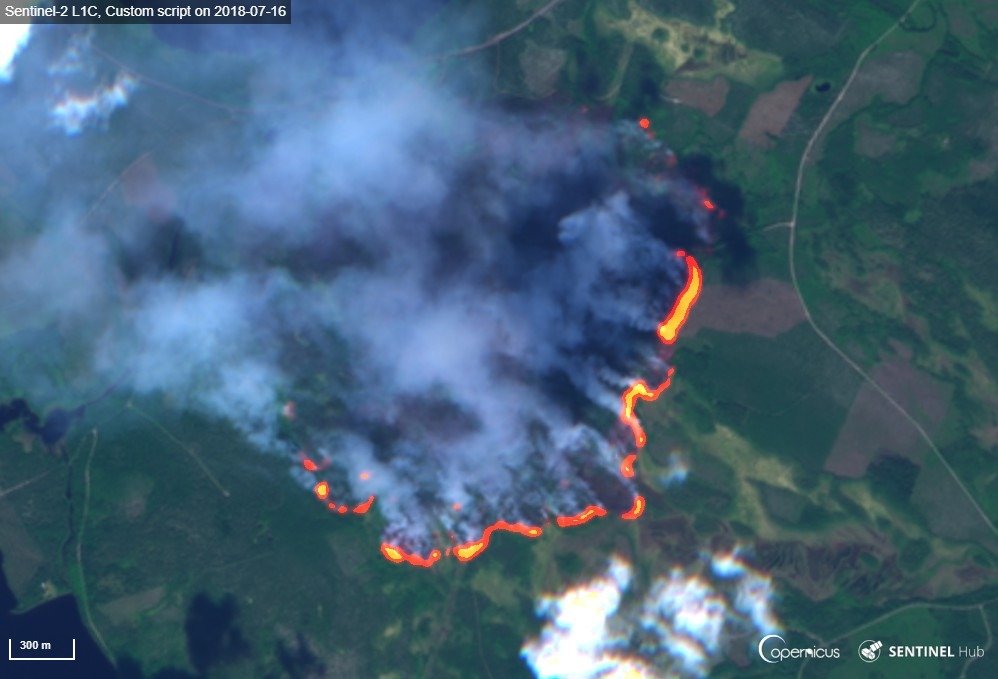
\includegraphics[scale=0.2]{fire.jpg}
\caption{Tipical forest fire.}
\label{fig:fire}
\end{figure}

The other optimizations where more subtle, and spotted thanks to the profiler,
but still contributed to shave of some time from the simulation. The first was
archived moving the calculation of $\beta_{ij}$ from the start of the simulation
loop to the end of it, in a conditional branch this because on most cells no
calculation has to be done and reading $\mathcal{F}$ would bring in its entire
cacheline, causing a probable miss.  Instead in this way it is calculated only
when needed and when the cache line was already loaded due to previous mandatory
calculations.

The second optimization was done precalulating $d$ and the sqare root in $f_w$,
because both can assume only two values, and finally rewriting the sum of sine
and cosine in a form where a single call to the sine function is made.

Before talking about those optimizations a little note about precalculating
functions has to be made, in modern day usually the bottle neck is not the
number of instructions to execute but the amout of memory that one has to acces,
therfore big tables of precalculated values are of no help.  But the ones
considered in my scenario are all tiny, in fact they all fit in a single
cacheline.

While $d$ is a relatively inexpensive value to calculte but it still contains a
call to libc and if the compiler is not smart enough could not be inlined, so
better to avoid this problem, the square root is a relatively expensive
operation espetially in a hot loop like this but the really slow function were
the sine and cosine calculations, those certainly cannot be avoided but can be
improved removing the two function call to sine and cosine and transforming them
in a single one to sine. The procedure is shown in table
\ref{tab:simplifications}. As a sidenote sine is also the same fuction called in
the Box-Muller transform to generate the normally distributed random numbers, so
that the sine code is always hot in the i-cache.

\begin{table}
\centering
\begin{tabular}{c c | c | c}
$\epsilon_1$ & $\epsilon_2$ & original equation & simplified equation\\
\hline
-1 & 1 & $-\cos(\alpha)+\sin(\alpha)$ & $-\sqrt{2}\sin(\frac{\pi}{4}-\alpha)$\\
0 & 1 & $\sin(\alpha)$ & $\sin(\alpha)$\\
1 & 1 & $\cos(\alpha) + \sin(\alpha)$ & $-\sqrt{2}\sin(\alpha+\frac{\pi}{4})$\\
-1 & 0 & $-\cos(\alpha)$ & $-\sin(\frac{\pi}{2}-\alpha)$\\
1 & 0 & $\cos(\alpha)$ & $\sin(\frac{\pi}{2}-\alpha)$\\
-1 & -1 & $-\cos(\alpha)-\sin(\alpha)$ & $-\sqrt{2}\sin(\alpha+\frac{\pi}{4})$\\
0 & -1 & $-\sin(\alpha)$ & $-\sin(\alpha)$\\
1 & -1 & $\cos(\alpha) + \sin(\alpha)$ & $\sqrt{2}\sin(\frac{\pi}{4}-\alpha)$\\
\end{tabular}
\caption{Simplifications}
\label{tab:simplifications}
\end{table}

\subsubsection{OpenMP}

The most effective optimization was the parallelization of the algorithm
together with the skip of cell that did not needed to be simulated. This
obvously because the algorithm is trivially parallelizable, due to the fact that
there is no need to comunication between the thread, except for the one at the
end of the for loop.

Because of this OpenMP allowed to easly and efficently parallelize the main loop
of the simulator. The only \texttt{pragma} used was the one in figure
\ref{fig:pragma}. Now let's explain it, the first part \verb+#pragma omp parallel for+
just tells OpenMP tho parallelize this for across the default number of cores
and equally divides the number of iterations to the number of default cores. The
\texttt{collapse(2)} just fuses the two nested loops into one.
\verb+default(none)+ \verb+firstprivate(rng_state)+
\verb+shared(s,Gamma,d,sqrt,funcs)+ are used to specify the visibility of the
variables outside the loop, the first one just tell to not use any default, so
that for every single variable we have to specify the sharing policy, the second
one gives a copy of the variable \verb+rng_state+ to each core and initializes
it to the same value in each of them, the third just sais that those variables
are shared among threads. Finally \verb+reduction(|: has_transmitted_fire)+ just
tels that at the end of the execution each thread all the prvate copies of
\verb+has_transmitted_fire+ shall be ORed together. This is done to efficiently
implement the halting condition avoiding problema like lock contetnio or false
sharing.

\begin{figure}
\centering
\footnotesize
\verb+#pragma omp parallel for collapse(2) default(none) firstprivate(rng_state)+
\verb+shared(s,Gamma,d,sqrt,funcs) reduction(|: has_transmitted_fire)+
\caption{OpenMP \texttt{pragma} used}
\label{fig:pragma}
\end{figure}

\subsection{Shell}

The POSIX shell \texttt{sh(1)}, togheter with its utilities, was used in the and
as the integration language between the two pieces of the simulator. It was used
expecially for its omnipresence in UNIX like systems, and my familiarity with
it.

\section{Experimental Results}%%%%%%%%%%%%%%%%%%%%%%%%%%%%%%%%%%%%%%%%%%%%%%%%%%

Now I am going to talk about the experimental results gathered during the
internship period. The primary experimental activity carried were software
testing and performance measuring.

\subsection{Goals}

The goals of the experiments done on the simulator software were to show the
correct execution of the single parts and the integration between the
database part of the simulator and the part that executes the model worked
correctly. Also a good level of performance had to be archived.

\subsection{Setting}

The majority of the testing and development was done on a machine running mac OS
Big Sur with an Intel Core i7 6 core processor. But for ensuring the corretc
execution in the Linux environment, where the program was supposed to run,
compilation and execution of workloads has also been done on Linux (and some
bugs have been discovered there exclusivelly).

On the software side of things two compilers have been used \texttt{clang(1)}
and \texttt{gcc(1)}, the profiler used was Apple's Instruments.app, the debugger
was \texttt{lldb(1)}. Both compiler supported various warnings and debbuging
fetures namely sanitizers. And the C language standard library offered the
\texttt{assert(3)} macro that was extensively used throughout the code.

\subsection{Correctness}

Correctness of the various parts of the software has been shown with mostly hand
generated test cases, and manual testing.

For the database schema testing various \texttt{INSERT}, \texttt{DELETE} and
\texttt{UPDATE} clauses have been tried to trigger all the varius check of the
data. No bogus data was able to get in the database after the testing was done.

C is a notoriously error prone language to program in, this includes
it's integer (and float) conversion, manual memory allocation,
undefined behavior and pointher arithmetic. But tools can help a
lot in producing good quality software.

For the execution part the majority of bugs where cought or reported via
warnings and the AddressSanitizer \cite{asan} feature of both \texttt{gcc(1)}
and \texttt{clang(1)}. During testing all the reported problems were solved and
no more were found. A special note has to be made about the few concurrency bugs
that were encountered all counght by setting \texttt{default(none)} in the
OpenMP \texttt{pragma}.

The only bugs that were not found by the previously mentioned tools in the model
executor, were logic ones related to the input validation.

The core part of the model executor was shown to be correct by inspeciton
because it is a relatively simple and straightforweard function, thanks in part
to OpenMP who handled all the parallelism in a clean and transparent way, and
allowed to test sequential and parallel code correctness commenting out just a
line of code.

\subsection{Computational Performances}

The non multicore optimizations save together more or less a second of execution
time as measured with \texttt{time(1)} (single core performance). Even though
they don't seem to be faster when analysed in isolation with Googlebench. I
think that this is realted to the use of the ports in the CPU but I haven't
verified this claim.

The parallel code is instead is roughly three times faster than the single core
one.

To give an idea of the level of performance reached by the final implementation
the current one is able to do 100 iterations on a grid of $1000\times 1000$
cell\footnote{The size of the state is 8MB and the one of the cells parameters
is 20MB bytes.}, taking a snapshot every 10, from a starting condidion where all
the cells are on fire, takes roughly 4.30s of real time including the file
reading.

% TODO: nell'implementatione e qua devo parlare dello skip e di quanto tempo salva.

\section{Conclusion}

In the end a correct and performant implementation of the simulator was
delivered, definatelly the hardest part of this intership did not came from the
development side but the software engeneering one. Having to take a imprecise
model and transforming it into a real programm was a real challenge. The
continous update and changes made it really difficult to actualy develop
something.

\subsection{Possible Improvements}

There are definatelly many things to improve. First of all the error handling
and the logging are a little bit messy. Than the part of code that dumps the
result of simulation to disk could be made to execute on separate threads, to
avoid pauses while running the simulation, but then the software will not be
anymore allocation free in the main loop, so a carefully designed allocation
stategy would have to be developed. Something like a pool allocator should be
good enough knowing that that the simulation state has alwas the same size.

Another optimization could be tried like the one proposed in the Game
Programming Graphics Black Book (citation), that are especially suited for
sparse cellular automata simulation. Also the use of \texttt{PREFETCH}
instructions could help.

\subsection{Future Work}

The execution part of the software could be rewritten as a library instead of
beeing a standalone program, because beeing written in C it is particularly
suited to be called by other languages (e.g. Java, Python etc\dots). To avoid
all the integration dance and concentrating directly in performat simulation.

A trivial version could be implemented on a GPU to see if the work saved by the
CPU implementation still makes it faster with respect to a GPU implementation.

\newpage

\appendix

\section{Description of the satellitar data}\label{sec:desc}

The values enumerated in the table \ref{tab:geo} are defined in the table
\ref{tab:forest}, \ref{tab:urbanization}, \ref{tab:water1}, \ref{tab:water2} and
\ref{tab:altimetry}.

\begin{table}
\centering
\begin{tabular}{|c|l|}
\hline
\textbf{Value} & \textbf{Class}\\
\hline
0 & Not forest\\
1 & Deciduous forest\\
2 & Coniferous forest\\
255 & External area\\
\hline
\end{tabular}
\caption{Forests}
\label{tab:forest}
\end{table}

\begin{table}
\centering
\begin{tabular}{|c|l|}
\hline
\textbf{Value} & \textbf{Class}\\
\hline
0 & Non waterproof zone\\
1 & Waterproof zone at 1\%\\
\vdots & \vdots\\
100 & Waterproof zone at 100\%\\
255 & External Area\\
\hline
\end{tabular}
\caption{Urbanization}
\label{tab:urbanization}
\end{table}

\begin{table}
\centering
\begin{tabular}{|c|l|}
\hline
\textbf{Value} & \textbf{Class}\\
\hline
0 & Dry soil\\
1 & Permanent water\\
2 & Temporary water\\
3 & Permanently wet\\
4 & Temporarely wet\\
253 & Sea cost water\\
255 & External area\\
\hline
\end{tabular}
\caption{Water 1}
\label{tab:water1}
\end{table}

\begin{table}
\centering
\begin{tabular}{|c|l|}
\hline
\textbf{Value} & \textbf{Class}\\
\hline
0 & Torrent absence\\
1 & Torrent presence\\
\hline
\end{tabular}
\caption{Water 2}
\label{tab:water2}
\end{table}

\begin{table}
\centering
\begin{tabular}{|c|l|}
\hline
\textbf{Value} & \textbf{Class}\\
\hline
0 & Minimum height\\
\vdots & \vdots\\
4380 & Maximum height\\
\hline
\end{tabular}
\caption{Altimetry}
\label{tab:altimetry}
\end{table}

\clearpage

\bibliographystyle{plain}
\bibliography{document} % TODO: cambiare il file in thesis.bib

\end{document}
